\documentclass[letter,12pt]{report}
\usepackage[utf8]{inputenc}
\usepackage[T1]{fontenc}
\usepackage[spanish, es-tabla]{babel}
\usepackage[sfdefault, condensed]{roboto}
\usepackage[margin=1cm]{geometry}
\usepackage{multicol,graphicx,fancyhdr,eso-pic,url,float,cite,lmodern,listings,times,textcomp, amsthm,amsmath,amssymb,dsfont,color,colortbl,sidecap,xspace,epic,eepic,anysize,setspace, hyperref, pdflscape,lscape}
\usepackage{blindtext}

%%%%%%Glosario
%\usepackage[acronym]{glossaries}
%\makeglossaries
%\renewcommand{\glossaryname}{Glosario}
%\renewcommand{\acronymname}{Acrónimos}


%\usepackage{apacite} %bibliografias Bibtex

%Tipos de Letra
%\renewcommand{\rmdefault}{phv} % Arial
\usepackage{mathptmx} %Times
%Margenes
\marginsize{3cm}{2cm}{2cm}{2cm}
\spacing{1}%interlineado

  \providecommand{\keywords}[1]{\textbf{\textit{Palabras Clave---}} #1}

\newcommand\BackgroundPic{ \put(-3,0){ \parbox[b][\paperheight]{\paperwidth}{ \vfill \centering 
\includegraphics[width=\paperwidth,height=\paperheight]{portada.jpg} \vfill }}} 
  
  %Definicion de Colores
\definecolor{gray97}{gray}{.97}
\definecolor{gray75}{gray}{.75}
\definecolor{gray45}{gray}{.45}
\definecolor{verdeo}{rgb}{0,.5,0.2}
\definecolor{listinggray}{gray}{0.9}
\definecolor{lbcolor}{rgb}{0.9,0.9,0.9}
\newcommand\gris[1]{\textcolor[gray]{.35}{\emph{#1}}}
\newcommand\rojo[1]{\textcolor[rgb]{1,0,0}{#1}}
\newcommand\blue[1]{\textcolor[rgb]{0,0,1}{{#1}}}
\newcommand\azul[1]{\textcolor[rgb]{0,0,1}{#1}}
\newcommand\verde[1]{\textcolor[rgb]{0,.5,0.2}{#1}}
\newcommand\naranjo[1]{\textcolor[rgb]{1.00,0.36,0.06}{\textbf{#1}}}
\newcommand\blanco[1]{\textcolor[rgb]{1,1,1}{\textbf{#1}}}
\newcommand {\red}[1]{\textcolor[rgb]{1.00,0.00,0.00}{#1}}
\newcommand\cita[1]{{\scriptsize \begin{flushright}\emph{(#1)}\end{flushright}}}
  

  
%%%Entornos de desarrollo
\newtheorem{ejemplo}{Ejemplo}
\newtheorem{definir}{Definición}
\newtheorem{prueba}{Prueba}
\newtheorem{demo}{Demostración}
\newtheorem{obs}{Observación}

\newcommand{\ignore}[1]{}
  
  %%%CODIGOS DE PROGRAMACION
\lstset{%backgroundcolor=\color{lbcolor},
	frame=Ltb, framerule=0pt, aboveskip=0.5cm, tabsize=4, rulecolor=, language=C, %%%CAMBIAR POR LENGUAJE DE PREFERENCIA
 stringstyle=\ttfamily,  %basicstyle=\footnotesize,
        upquote=true, aboveskip={1.5\baselineskip}, columns=fixed, showstringspaces=false, extendedchars=true,breaklines=true, prebreak = \raisebox{0ex}[0ex][0ex]{\ensuremath{\hookleftarrow}}, showtabs=false, showspaces=false, showstringspaces=false,
        %tipos de letra y colores
        identifierstyle=\ttfamily,
        keywordstyle=\bfseries  \color[RGB]{0,2,216}, %palabras reservadas
        commentstyle= \scriptsize\color[rgb]{0,.5,0.2}, %comentarios
        stringstyle=\color[RGB]{216,0,114},%cadena de texto
        %numeracion de lineas
        framextopmargin=3pt, framexbottommargin=3pt, framexleftmargin=0.4cm,
        framesep=0pt, rulesep=.4pt, rulesepcolor=\color{black}, numbers=left, numbersep=15pt, numberstyle=\tiny, numberfirstline = false, breaklines=true,literate={á}{{\'a}}1 {é}{{\'e}}1 {í}{{\'i}}1 {ó}{{\'o}}1 {ú}{{\'u}}1
  {Á}{{\'A}}1 {É}{{\'E}}1 {Í}{{\'I}}1 {Ó}{{\'O}}1 {Ú}{{\'U}}1
  {à}{{\`a}}1 {è}{{\`e}}1 {ì}{{\`i}}1 {ò}{{\`o}}1 {ù}{{\`u}}1
  {À}{{\`A}}1 {È}{{\'E}}1 {Ì}{{\`I}}1 {Ò}{{\`O}}1 {Ù}{{\`U}}1
  {ä}{{\"a}}1 {ë}{{\"e}}1 {ï}{{\"i}}1 {ö}{{\"o}}1 {ü}{{\"u}}1
  {Ä}{{\"A}}1 {Ë}{{\"E}}1 {Ï}{{\"I}}1 {Ö}{{\"O}}1 {Ü}{{\"U}}1
  {â}{{\^a}}1 {ê}{{\^e}}1 {î}{{\^i}}1 {ô}{{\^o}}1 {û}{{\^u}}1
  {Â}{{\^A}}1 {Ê}{{\^E}}1 {Î}{{\^I}}1 {Ô}{{\^O}}1 {Û}{{\^U}}1
  {œ}{{\oe}}1 {Œ}{{\OE}}1 {æ}{{\ae}}1 {Æ}{{\AE}}1 {ß}{{\ss}}1
  {ű}{{\H{u}}}1 {Ű}{{\H{U}}}1 {ő}{{\H{o}}}1 {Ő}{{\H{O}}}1
  {ç}{{\c c}}1 {Ç}{{\c C}}1 {ø}{{\o}}1 {å}{{\r a}}1 {Å}{{\r A}}1
  {€}{{\EUR}}1 {£}{{\pounds}}1 {Ñ}{{\~N}}1 {ñ}{{\~n}}1 {¿}{{?`}}1
}
%%%%FIN CODIGOS DE PROGRAMACION
\def\figurename{}
  
%%%%%%%%%%ENCABEZADO Y PIE DE PAGINA
%encabezado de las paginas pares e impares.
\rhead[PP]{Ingeniería Civil en Informática}
\renewcommand{\headrulewidth}{0.5pt}
%pie de pagina de las paginas pares e impares.
\lfoot[nombre]{Muñoz Viveros}
\rfoot[rut]{Universidad de los Lagos}
\renewcommand{\footrulewidth}{0.5pt}
%encabezado y pie de pagina de la pagina inicial de un capitulo.
\fancypagestyle{plain}{
\fancyhead[R]{Ingeniería Civil en Informática}
\fancyfoot[L]{Muñoz Viveros}
\fancyfoot[R]{Universidad de los Lagos}
\renewcommand{\headrulewidth}{0.5pt}
\renewcommand{\footrulewidth}{0.5pt}
}
\pagestyle{fancy} 
%%%%%%%%%%FIN ENCABEZADO Y PIE DE PAGINA 

\begin{document}

%%%%%%%%%%%PORTADA%%%%%%%%%%%%%%%%%%%%%
\setlength{\unitlength}{1 cm} %Especificar unidad de trabajo
\thispagestyle{empty}

\AddToShipoutPicture*{\BackgroundPic}

   \title{\scshape\Huge{Detección de presencia de parásitos en examen
parasitológico seriado de deposiciones con visión por computadora}\\\vspace{1cm}
        \Large Departamento de Ciencias de la Ingeniería\\
        \Large Ingeniería Civil en Informática\\
        \large Campus Puerto Montt, Chile}
   \author{
      Diego Ignacio Muñoz Viveros\\
      diegoignacio.munoz@alumnos.ulagos.cl
   }
   \date{Profesor Guía: Joel Sebastian Torres Carrasco\\  Co-guía: Carlos Dupré Alvarado\\
   \today}
   \maketitle
   \ClearShipoutPicture


\cleardoublepage
\pagenumbering{roman}
\setcounter{page}{1}

%%%%Agradecimientos
\chapter*{Agradecimientos}
Gracias

%%%%%%%%RESUMEN
\begin{abstract}
    El examen parasitológico seriado de deposiciones es un examen realizado para la
    detección de presencia parasitológica en pacientes. El examen se lleva a cabo con la
    toma de muestras de deposiciones del paciente y posteriormente se hace observación de
    las mismas por medio de microscopio, en la realización de la observación se documenta
    la confirmación y clasificación de presencia parasitológica en orden de dar con un
    tratamiento certero, eficaz y acorde a las detecciones.

    El uso de la visión por computadora espera demostrar el aumento en la precisión y
    velocidad de la detección y clasificación de parásitos con objetivo de reducir
    incertidumbre y error humano introducido en la observación manual ejercida en el
    proceso de observación del examen parasitológico seriado de deposiciones. La visión
    por computadora es la combinación de tecnologías que permite a las computadoras
    generar inferencia respecto a imágenes estáticas o en movimiento emulando la visión
    humana por medio de un aprendizaje basado en conjuntos de datos utilizados como
    ejemplos iniciales de los cuales el modelo generado ajustará sus parámetros.

    En el presente trabajo, se realizó una búsqueda de conjuntos de datos sobre parásitos,
    se desarrolló un modelo de clasificación de imágenes basados en visión por computadora y
    se probaron diferentes alternativas para mejorar la calidad de la identificación y la 
    clasificación.

    Finalmente, este trabajo aporta un marco experimental sobre un conjunto de datos acotado
    de parásitos, que puede ser liberado a producción, ampliando la cantidad de parásitos a
    identificar.

%Resume en un (1) párrafo el contenido del informe en un máximo de 350 palabras.
%Debe ser preciso:
%\begin{itemize}\justifying
  %\item Establece el problema
  %\item Dice porqué es interesante
  %\item Señala los logros y desafios
%\end{itemize}
%Un resumen debe ser llamativo, motivador, descriptivo y sin contenido específico. \textbf{No incluye}: citas, referencias, conclusiones, figuras ni tablas.
%
%
\keywords{Parasitólogia, Serializado, Deposiciones, Visión por Computadora, Modelo,
Conjunto de Datos, \textit{Underfiting}, \textit{Overfiting}}
\end{abstract}


%%%%%%INDICES
\tableofcontents
%\listoffigures
%\renewcommand{\listtablename}{Índice de tablas}
%\listoftables
%\renewcommand{\lstlistlistingname}{Índice de algoritmos}
%\lstlistoflistings
%\addcontentsline
%%%%%%%%%%%%%FIN PORTADA%%%%%%%%%%%%%%%%

\cleardoublepage
\pagenumbering{arabic}
\setcounter{page}{1}

%%%%%%%%COMIENZO



\chapter{Introducción}\label{intro}
% Todavía hay gran cantidad de exámenes echos a mano
% Hacer esto a mano no suple la demanda médica
    En la actualidad en los laboratorios médicos existen gran cantidad de exámenes
    relacionados a la observación microscopica de muestras, estos exámanes son ralizados
    bajo observación humana de manera totalmente manual. Normalmente los exámenes que
    involucran esta observación microscopica suelen demandar bastante tiempo por muestra,
    esto multiplicado a la demanda habitual en el área de la salud nos da a conocer una
    problemática relacionada a la incapacidad de suplir la demanda en un tiempo
    pertinente.

% Sesgo humano
% Certeza incierta
    Otra característica inerente a la observación está relacionada al error humano
    introducido en las observaciónes, resultando en observaciones con clasificaciones
    erroneas, esto concluyendo en el mal diagnostico médico. En ocaciones puede haber una
    gran diferencia entre las observaciones de distintos tecnólogos médicos sobre la
    misma muestra, esto en resumen, agrega gran incertidumbre a los análisis que
    normalmente solo puede ser resuelta con observaciones adicionales o complementarias.

% Introducción del rol de la tecnología médica
% Intro a nuestro laboratorio clínico cesfam de hornopiren
% Dentro de los exámenes con mirada experta
    La tecnología médica en el ámbito del conocimiento abarca el estudio e investigación
    que tiene como objetivo la aplicación de diferentes tipos de tecnologías para mejorar
    la salud de las personas durante su diagnóstico, desarrollo de la enfermedad y
    tratamiento aplicado. En el contexto médico, la tecnología médica es la rama de la
    salud que involucra a profesionales que se forman en los avances tecnológicos para
    aplicarlos a la medicina y las ciencias de la salud. %citar acá

%TODO: revisar
    Para la consultoria de este trabajo se cuenta con la ayuda del laboratorio clínico
    CESFAM de Hornopiren, con la ayuda del tecnólogo médico y jefe del laboratorio
    clínico Carlos Dupré Alvarado.

    El examen parasitológico seriado de deposiciones es un examen realizado para la
    detección de presencia parasitológica en pacientes. El examen se lleva a cabo con la
    toma de muestras de deposiciones del paciente y, posteriormente, se hace observación
    de las muestras por medio de observación microscopica, en la realización de la
    observación se documenta la confirmación y clasificación de presencia parasitológica
    en orden de dar con un tratamiento certero, eficaz y acorde a las detecciones. %cita aqui
    La denominación seriado refiere a las condiciones en las que estas muestras, tres
    muestras enfrascadas por separado, serán tomadas con la finalidad de tener muestras
    en distintos ciclos larvales.

% Cual es el problema que tenemos acá
% Inconsistencia en las mediciones / definición del problema
    El problema es que dado lo extenuante de la observación y lo altamente susceptible a
    sesgo del observador el examen es muy sensible a perdida o mala clasificación de
    avistamientos llevando a malos diagnósticos médicos. En este trabajo se propone una
    solución inteligente para automatizar el examen parasitológico seriado de
    deposiciones para poder mejorar la calidad de los resultados y así mejorar la calidad
    de vida de las personas.

    Para realizar este proyecto se pretende usar tecnologías que permitan aprovechar la
    experiencia de los tecnólogos médicos y utilizarla para crear mejores resultados.
    Es por ello que se pretende utilizar tecnologias de visión por computadora para
    automatizar la observación de muestras y a su vez reducir el grado de error mientras
    se apunta a una implementación rápida y simple.

    La visión por computadora es la combinación de tecnologías que permite a las
    computadoras generar inferencia respecto a imágenes estáticas o en movimiento
    emulando la visión humana por medio de un aprendizaje basado en conjuntos de datos
    utilizados como ejemplos iniciales de los cuales el modelo generado ajustará sus
    parámetros. %cita acá
    El uso de la visión por computadora espera demostrar el aumento en la precisión y
    velocidad de la detección y clasificación de parásitos con objetivo de reducir
    incertidumbre y error humano introducido en la observación manual ejercida en el proceso
    de observación del examen parasitológico seriado de deposiciones. 

% El gran desafió tésnico
% Uno de los problemas, existencia de dataset relacionados al examen
    El desafío técnico encontrado está relacionado a la estructuración de un conjunto de
    datos de imágenes microscopicas que contengas la información suficiente para generar
    un modelo robusto y de altas prestación con gran capacidad de generalización para el
    examen parasitologico seriado de deposiciones.

% Continua que se verá

\chapter{Marco Teórico}\label{teorico}

\section{Parasitología}
\subsection{Definición}
La parasitología es la rama de las ciencias biologicas dedicada a el estudio de
organismos, denominados parásitos, que dependen de otro para poder sobrevivir y que
ocasionan grandes daños a las especies de las cuales dependen, relación llamada
parasitismo.

La parasitología es una disciplina con aplicación en campos variados como medicina,
farmacologia y veterinaria. Es utilizada en la investigación de parásitos que pueden
producir enfermedades en plantas y animales con objeto de analizar, diagnosticar y
posteriormente establecer un tratamiento óptimo para poder curarlas y erradicarlas.

Gran parte de los parásitos más dificil de tratar son los que se alojan en el
interior del organismo, lo que puede ingresar por via oral o fluidos y gran parte de
estos pueden alojarse en el sistema digestivo, principalmente en estomago e
intestino.

En el contexto de la medicina, la área de \textbf{Tecnología Médica} en su
especialización de parasitología esta encargada de la realización y analisis de
exámenes con la finalidad de diagnosticar amenazas relacionadas a la disciplina.

\subsection{Exámenes parasitologicos}

Existen muchos tipos de análisis de laboratorio para diagnosticar enfermedades parasitarias.
El tipo de análisis que solicite el médico se basará en sus signos y síntomas presentados
durante la consulta médica, cualquier otra afección médica que pueda tener y sus
antecedentes de viajes.

El análisis de laboratorio se lleva a cabo con las observaciones de muestras entregadas
al laboratorio por el médico tratante. Estas muestras dependen de la busqueda de los
parásitos sospechados y sus posibles ubicaciones, siendo estas muestras de la forma de
sangre, heces, muestras urogenitales, esputo, aspirados o biopsias. La especificidad de
los exámanes puede variar en la capacidad de detectar diferentes especies o realizar
busquedas de manera particular.

Estos exámenes se pueden dividir en dos categorias:

\begin{itemize}
    \item Invasivos: la adquisición de la muestra requiere intervención
        quirurgica algún tipo como las biopsias.
    \item No invasivos: la toma de la muestra presenta un método de obtención que no
        involucra una intervención invasiva al paciente como serían muestras de sangre o
        heces.
\end{itemize}

\subsection{Procedimiento de exámenes}

Para la realización de los exámenes se procede de las siguientes formas: %cita acá

\begin{enumerate}
    \item \textbf{Exámenes de muestra de sangre}: la muestra es tintada y analizada por
        goteo grueso y/o fino con un microscopio. El goteo fino es una forma de repartir
        la muestra en un portaobjeto \footnote{Placa de acrílico trasparente usada para
        manejo de muestras para microscopio} a manera de dejar una capa delgada y
        uniforme en la cual realizar observasiones, el goteo grueso por otro lado,
        consiste en soltar una gota de muestra de forma que la tensión superficial de la
        muestra mantenga su forma circular para dejar decantar las celulas contenidas en
        la muestra al fondo.  La tinción es el proceso en el cual se suman compuestos a
        la muestra que reaccionan a componentes conocidos con el fin de teñir componente
        para facilitar la visualización.
    \item \textbf{Endoscopia/Colonoscopia}: Conciste en la insersión en la boca
        (endoscopia) o el recto (colonoscopia) de una sonda con la cual el médico,
        normalmente un gastroenterólogo, examina las cavidades en busca de presencia
        parasitaria y/o lesiones de caracter aludible a presencia parasitaria.
    \item \textbf{Exámenes parasitológico seriado de deposiciones}: consiste en el
        análisis de tres muestras seriadas \footnote{Muestras tomadas con intervalos de
        tiempo equidistantes con objetivo de muestrear sin que se pierdan ciclos
        larvarios evitando excluir avistamientos} de heces tintadas con observación por
        microscopio . La observación se realiza por goteo fino.
    \item \textbf{Resonancia Magnética (RM), Tomografía axial computarizada (TAC)}:
        Pruebas ralizadas para buscar enfermedades parasitarias que pueden provocar
        lesiones en los órganos.
\end{enumerate}

\subsection{Examen Parasitológico Seriado de Deposiciones}
% Que es, para que, procedimiento
% Hablar del contexto del tecnologo medico
Como se menciona anteriormente, el examen parasitológico seriado de deposiciones es un
examen que busca estudiar la presencia parasitaria intestinal por medio de observaciones
de muestras de heces. La realización de este examen es llevado a cabo por un tecnólogo
médico y su principal objetivo es documentar las observaciones realizadas.

La realización del examen en detalle se muestra a continuación:
\begin{enumerate}
    \item Una vez se reconoce la necesidad de la realización del examen, el médico
        trantante pedirá la preparación de tres frascos de muestras con 10-20 ml de
        liquido fijador\footnote{Liquido conservantes, normalmente formaldehído}.
    \item Se hace entrega al paciente de los frascos junto a una nota con las
        instrucciones para la toma de muestras, conservación de las mismas y precauciones
        a tomar.
    \item Cuando se reciben las muestras y se valida su tamaño, los tiempos en los que se
        tomaron y la forma en que se conservaron, estas pasaran a ser entragadas al
        laboratorio donde seran almacenadas y/o examinadas.
    \item Las muestras son retiradas del área de refrigeración, en el caso que se
        ecuentren en concervación, y se proceden a intruducir una porción de cada frasco
        en tres probetas diluidas en el liquido fijador.
    \item Se centrifugan las muestras en orden de separar el material fecal del liquido
        fijador para poder extraerlo.
    \item En caso de que el tecnólogo lo considere necesario, tintar la muestras con
        soluciones reactivas que resalten componentes especificos para facilitar las
        observaciones.
    \item Dejar caer una gota de cada una de las muestras en un portaobjeto y esparcir
        para observación de goteo fino.
    \item Hacer observación de las muestras con gran detalle en el microscopio y
        documentar hallazgos en caso de haber.
    \item En caso de no detectar presencia parasitaria, documentar que no se observa
        presencia en la muestra.
\end{enumerate}

Para la correcta realización del examen existen ciertas consideraciones expuestas a
continuación:
\begin{itemize}
    \item La toma de muestras debe avarcar un período mínimo de cinco días.
    \item La duración de la observación microscópica puede durar al rededor de 45
        minutos y es dependiente de la habilidad y experiencia del tecnólogo.
    \item En caso de encontrar alguna anormalidad en la recepción de las muestras por
        parte del paciente, se debe pedir que este haga la toma nuevamente en frascos
        diferentes.
    \item La muestra que no se utilice durante la observación deber ser concervada en
        refrigeración.
    \item En caso de existir dudas sobre la observación de las muestras, se puede
        realizar una segunda observación.
\end{itemize}

\section{Visión por Computadora}
% Definición
La visión por computadora es el campo de la inteligencia artificial (IA) que permite a
los computadores y sistemas derivados a extraer información util de imagenes digitales,
videos y otras entradas visuales y tomar actiones o hacer recomendaciones basadas en esta
información. Si la IA permite a los computadores pensar, la visión por computadora les
permite ver, observar y entender. %cita acá

La visión por computadora, así como muchas otras ramas de la disciplica de IA, logra la
tarea de inferir gracias al aprendizaje de máquinas. El aprendizaje de maquinas consiste
en el entrenamiento de modelos de IA en base a conjuntos de datos que harán que los
distintos modelos aprendan a reconocer patrones y generen la lógica interna necesaria
para permitirles inferir de manera correcta.

% Metodología de cs (Data augmentation, Data cleaning, Balancing)
\subsection{Conjunto de Datos}
El manejo de los conjuntos de datos es una de las tareas más importantes a la hora de
diseñar un modelo de IA, ya que la información y como esté clasificada marcará como el
modelo podrá desempeñarse en un entorno de uso general o específico que no contenga
información vista con anterioridad.

La estructura general de un conjunto de datos en modelos de visión por computadora suele
consistir en un conjunto de imagenes o videos junto a etiquetas que muestran la
información contenida en estas, normalmente en la forma de coordenadas que delimitan el
área en donde se localiza en la imagen el objeto a identificar y/o clasificar, junto a la
etiqueta que identifíca que es o que acción esta ocurriendo.

Es importante contar con un conjunto de datos que contenga gran cantidad de ejemplos
relacionados a la tarea que se espera lograr, esto con objetivo de generalizar los
patrones e información obtenida por parte del modelo durante el proceso de entrenamiento.
La cantidad de información que se requiera estará dada por la complejidad en el modelo a
entrenar y la complejidad de la tarea a desarrollar, y el análisis de estos parámetros
dependerá del equipo de desarrollo. Cuando en entrenamiento carece de un conjunto de
datos contundente o el modelo es muy simple para la tarea ocurre \textit{underfiting},
esto es, cuando el modelo realiza inferencias escazas y/o erroneas.

Para un hacer buen provecho de la información existen diferentes tratamientos realizables
a los conjuntos de datos como lo son el limpieza de datos, aumento de datos y el balanceo
de datos.

\subsubsection{Limpieza de Datos}
\subsubsection{Aumento de Datos}
\subsubsection{Balanceo de Datos}

% Modelos de cv
% Segmentación
% Tipo de imágenes (microscópicas)

\section{Estado del Arte}\label{arte}
% Alternativas preexistentes
% Conjuntos de datos preexistentes

\chapter{Formulación del Proyecto}\label{formulación}

\section{Objetivo General}
Crear un modelo de aprendizaje de maquinas para la detección de y clasificación de
parásitos en el análisis parasitológico de seriado de deposiciones.

\section{Objetivos Específicos}
\begin{enumerate}\justifying
    \item Recopilar y estructurar un conjunto de datos de imágenes de muestras para el entrenamiento y testeo del modelo de detección de parásitos.
  \item Definir un modelo de detección de parásitos para la automatización de resultados del examen parasitológico seriado de deposiciones basado en visión por computadora.
  \item Analizar y validar la calidad de las predicciones de la detección de parásitos en las muestras, a través de experimentación con el conjuntos de datos recopilado y con muestras obtenidas desde procedimientos reales del examen parasitológico seriado de deposiciones, utilizando imagenes microscopicas.
\end{enumerate}

\section{Justificación}
%Que se planea realizar y hasta que punto se espera llegar.
%
%Esta subdivisión debe:
%\begin{enumerate}\justifying
  %\item Identifique el producto del software para ser diseñado por el nombre (por ejemplo, Anfitrión DBMS, el Generador del Reporte, etc.);
  %\item Explique eso que el producto (del software hará y que no hará.
  %\item Describe la aplicación del software especificándose los beneficios pertinentes, objetivos, y metas;
  %\item Sea consistente con las declaraciones similares en las especificaciones de niveles superiores (por ejemplo, las especificaciones de los requisitos del sistema), si ellos existen.
%\end{enumerate}
\blindtext

\section{Metodología}
\begin{enumerate}\justifying
    \item Recopilar y estructurar un conjunto de datos de imágenes de muestras para el entrenamiento y testeo del modelo de detección de parásitos.
        \begin{enumerate}
            \item Revisión de conjunto de datos disponibles relacionados al examen
                parasitológico seriado de deposiciones.
            \item Definir una estructura estandar para almacenar imagenes microscopicas
                de examen parasitológico seriado deposiciones.
            \item Implementar un procedimiento de extracción y limpieza de imagenes de
                examen parasitológico seriado de deposiciones.
            \item Realizar un procedimiento de análisis exploratorio de datos.
        \end{enumerate}

  \item Definir un modelo de detección de parásitos para la automatización de resultados del examen parasitológico seriado de deposiciones basado en visión por computadora.
      \begin{enumerate}
          \item Adoptar una metodología (elección de experimento, metricas, configuración
              y \textit{kfolds}) de proyectos de visión por computadora para relizar una
              comparación de la calidad de los modelos.
          \item Proponer distintos modelos para la detección de parásitos en imagenes
              microscopicas.
          \item Seleccionar el o los modelos con mejor calidad de resultado.
      \end{enumerate}

  \item Analizar y validar la calidad de las predicciones de la detección de parásitos en las muestras, a través de experimentación con el conjuntos de datos recopilado y con muestras obtenidas desde procedimientos reales del examen parasitológico seriado de deposiciones, utilizando imagenes microscopicas.
      \begin{enumerate}
          \item Implementar la metodología elegida o adaptada para el tratamiento de
              imagenes microscopicas.
          \item Implementar el procedimiento de predicción de parásitos detectada en las
              imagen microscopicas.
          \item Implementar el reporte final de parásitos detectados en las muestras a
              través del modelo de visión por computadora.
          \item Recopilación de nuevas muestras, sus resultados, su validación y la
              retroalimentación del tecnologo médico.
      \end{enumerate}
\end{enumerate}

%\subsubsection{Equipo de Trabajo}
%Content ;v
% Calza esto
% 1
% 2-3.5
% 3-4

\subsection{Planificación}
\begin{figure}[H]
    \centering
    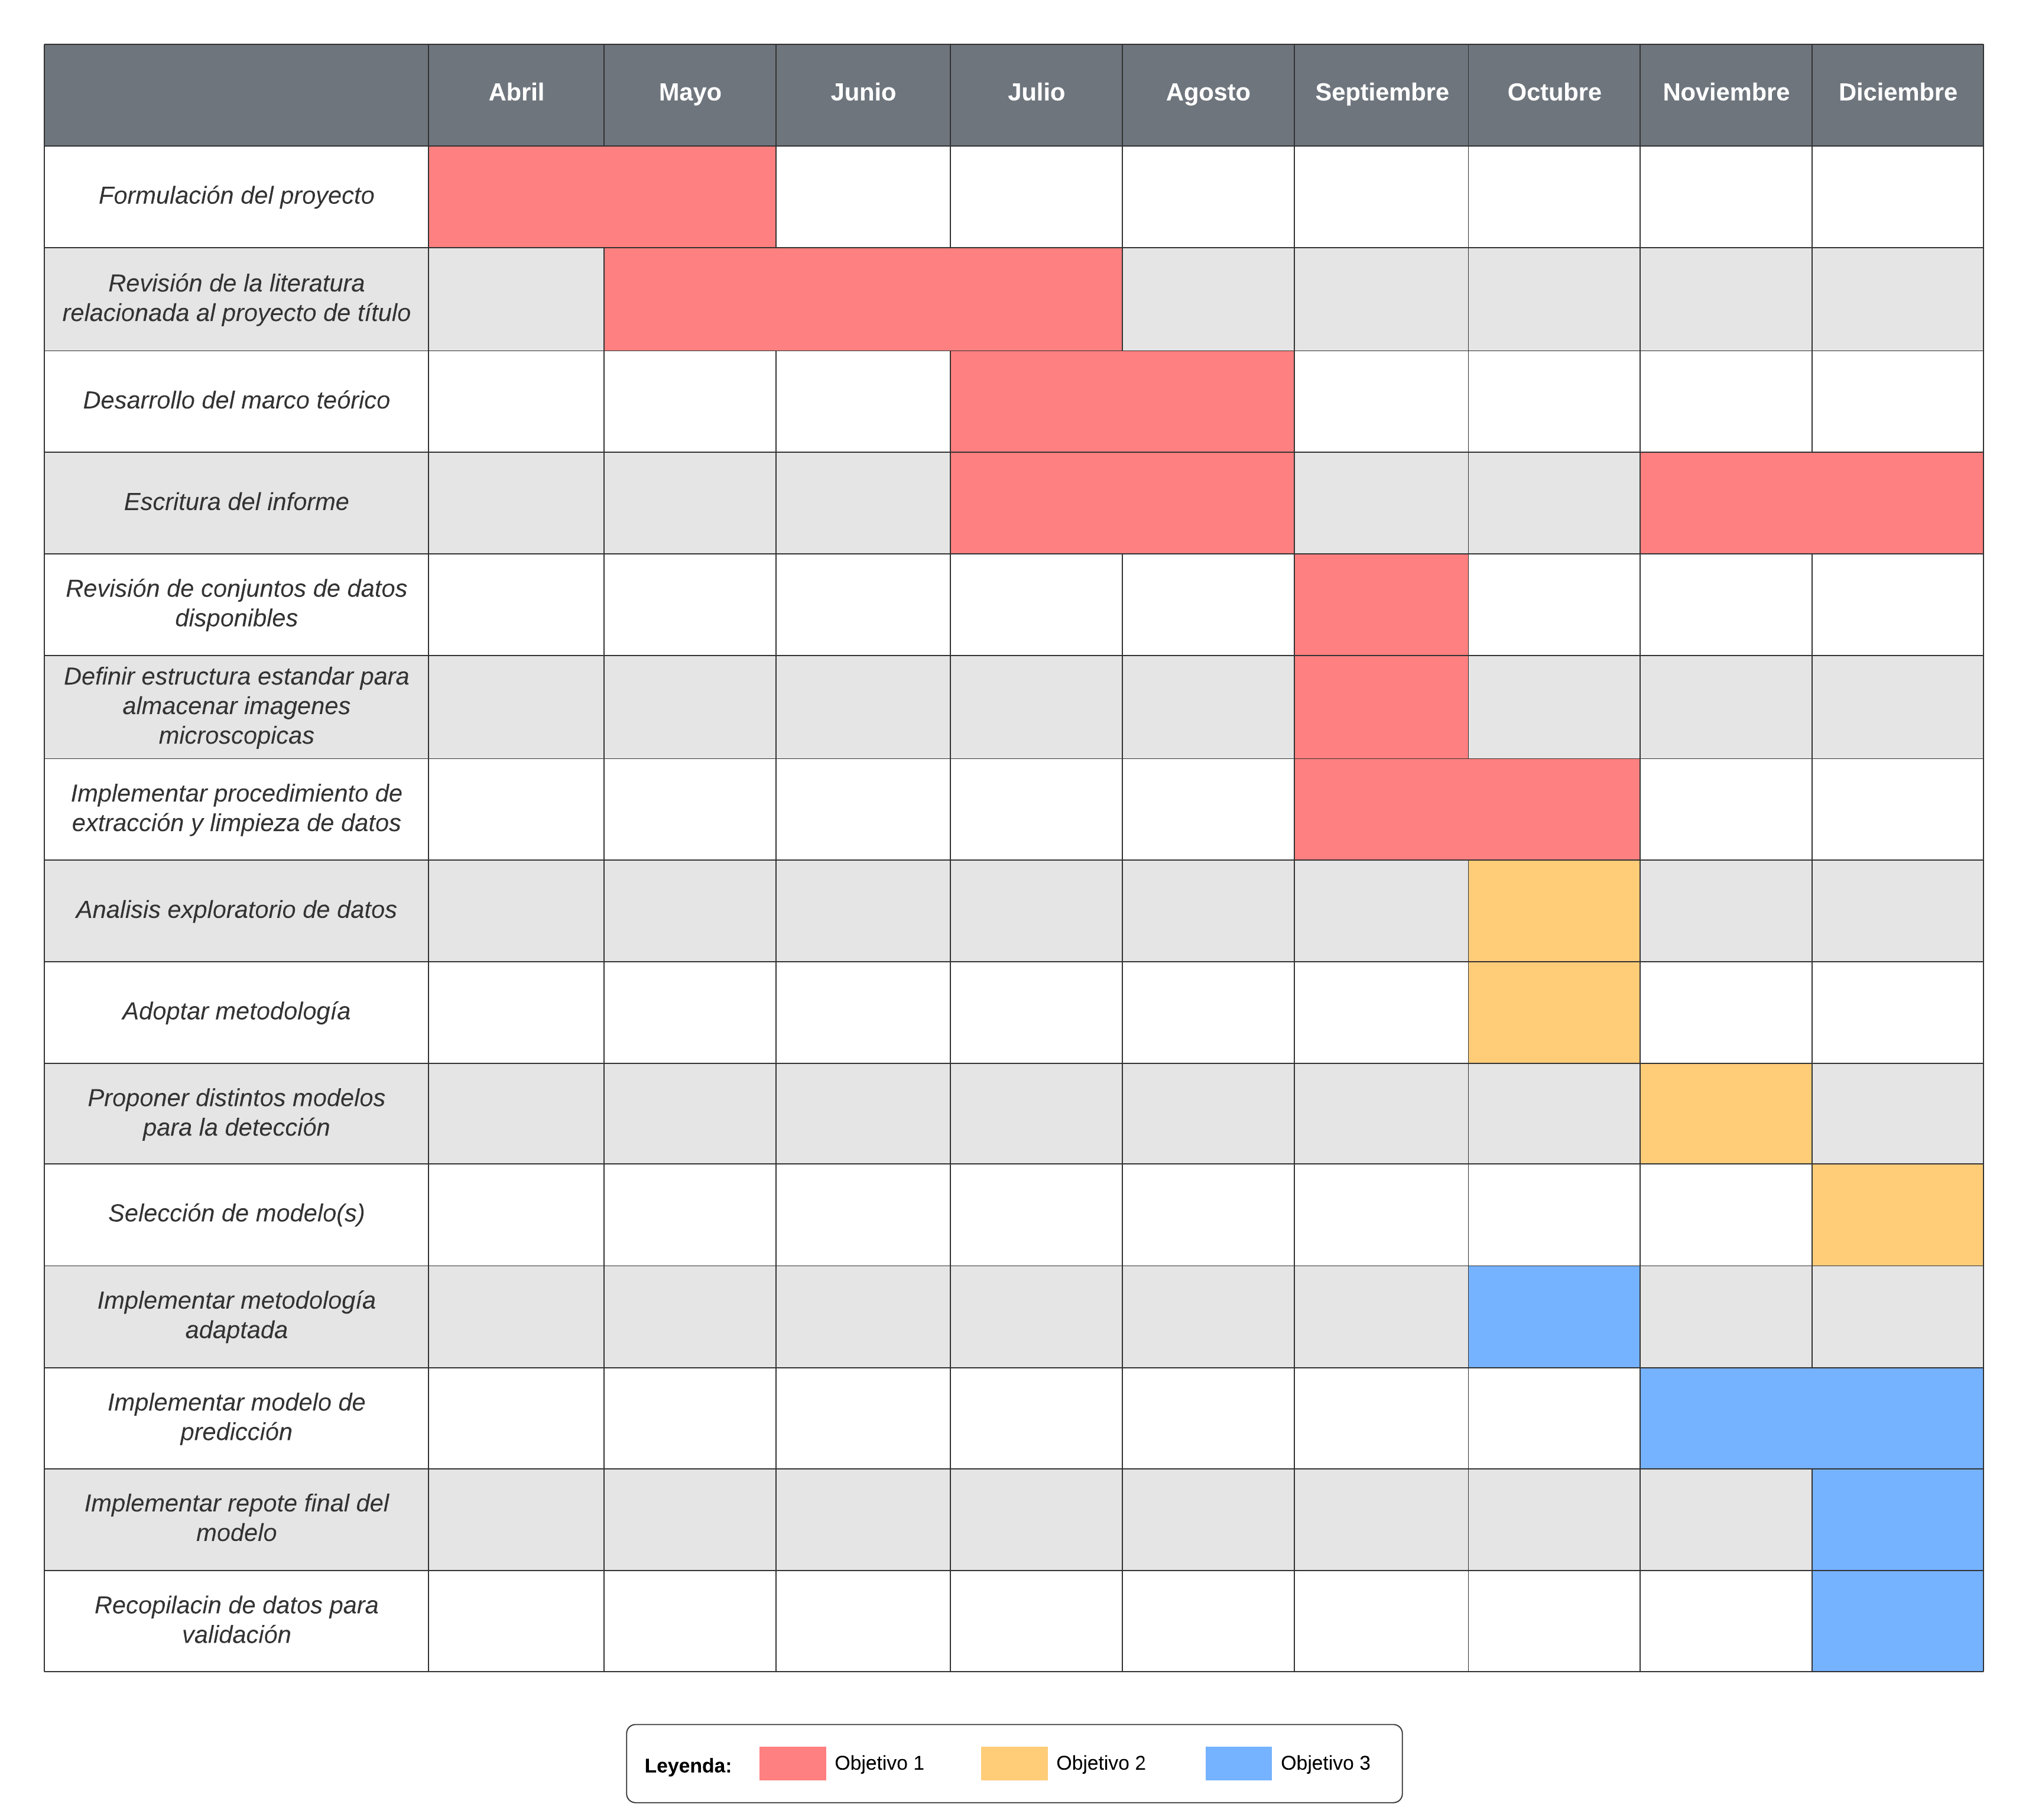
\includegraphics[width=0.9\textwidth]{gantt}
    \caption{Carta Gantt para desarrollo del proyecto}
    \label{fig:gantt}
\end{figure}

%\subsection{Desglose de Actividades}\label{PERT}
%En esta sección se describen cada una de las actividades, duración, dependencias, caminos críticos, entre otras y se debe dar una conclusión de lo mismo.
%\begin{figure}[hbt]
%\begin{tabular}{|c|c|c|c|c|}\hline
  %\textbf{Actividad}&\textbf{Duración} &\textbf{Después de} & \textbf{Simultanea} & \textbf{Antes de}\\\hline
%& & &&\\\hline
%
%\end{tabular}
  %\caption{Duración de tareas y dependencias}
%\end{figure}
%
%\begin{landscape}
%\begin{figure}[hbt]
  %\centering
  %%\includegraphics{}
  %\caption{Grafo de Actividades del Proyecto XYZ}
  %\label{CPM}
%\end{figure}
%\end{landscape}
%
%\begin{landscape}
%\begin{figure}[hbt]
  %\centering
  %%\includegraphics{}
  %\caption{Grafo de Actividades con duración del Proyecto XYZ}
  %\label{CPMduracion}
%\end{figure}
%\end{landscape}
%
%\begin{figure}[hbt]
 %\begin{tabular}{|c|c|cc|cc|c|c|}\hline
 %& & \multicolumn{2}{|c|}{\textbf{Inicio}} & \multicolumn{2}{|c|}{\textbf{Termino}} & \textbf{Holgura} & \\
%\textbf{Actividad}& \textbf{Duración}& \textbf{Temprano} &\textbf{Tardío} &\textbf{Temprano} &\textbf{Tardío} &\textbf{Total}  &\textbf{Crítico} \\\hline
%& & &   & &   & & \\\hline
%
%\end{tabular}
  %\caption{Cálculo del diagrama de actividades}
%\end{figure}
%
%\begin{landscape}
%\begin{figure}[hbt]
  %\centering
  %%\includegraphics{}
  %\caption{Grafo de Actividades con duración y caminos críticos}
  %\label{CPMcritico}
%\end{figure}
%\end{landscape}

\chapter{Conclusión}\label{conclusion}
En las conclusiones se destaca lo mostrado en el trabajo, resaltando los resultados. Se indican los trabajos futuros. Usualmente, luego de las conclusiones se incluye un párrafo de agradecimientos a quienes auspician la investigación.
\section{Principales aportes}
\section{Contraste de resultados}
%\section{Trabajos futuros} Solo si corresponde.

%%%%%REFERENCIAS
\renewcommand{\refname}{Referencias}

%agregar referencias
\bibliographystyle{apalike}\bibliography{document.bib}

\renewcommand{\appendixname}{Anexos}
\appendix

\chapter{Definciones, Acronimos y Abreviaturas}\label{definiciones}
\section{Definiciones}
\section{Acrónimos}
\section{Abreviaturas}

\chapter{Configuraciones}\label{configuracion}
\blindtext %reemplazar esta linea

\chapter{Anexo de Código}\label{codigoA}
\lstset{language=SQL}
   \vspace{-0.8cm}
\begin{lstlisting}
-- Database: acuario

-- DROP DATABASE acuario;

CREATE DATABASE acuario
  WITH OWNER = postgres;


CREATE TABLE especies(
    sno integer PRIMARY KEY,
    nombre character varying(20),
    alimento character varying(20)
);

CREATE TABLE tanques(
    tno integer PRIMARY KEY,
    nombre_tanque character varying(20),
    color_tanque character varying(20),
    volumen  integer NOT NULL
);

CREATE TABLE peces(
    pno integer PRIMARY KEY,
    nombre_peces character varying(20),
    color_peces character varying(20),
    tno integer NOT NULL,
    sno integer NOT NULL,
    FOREIGN KEY (tno) REFERENCES tanques (tno) ON UPDATE CASCADE ON DELETE CASCADE,
    FOREIGN KEY (sno) REFERENCES especies (sno) ON UPDATE CASCADE ON DELETE CASCADE
);

CREATE TABLE eventos(
    eno integer PRIMARY KEY,
    pno integer NOT NULL,
    fecha date,
    FOREIGN KEY (pno) REFERENCES peces (pno) ON UPDATE CASCADE ON DELETE CASCADE
);



INSERT INTO especies VALUES(17,'delfin','arenque');
INSERT INTO especies VALUES(22,'tiburon','cualquier cosa');
INSERT INTO especies VALUES(74,'olomina','gusano');
INSERT INTO especies VALUES(93,'ballena','mantequilla de mani');
INSERT INTO especies VALUES(100,'pez espada','gusano');
INSERT INTO especies VALUES(120,'pez globo','gusano');

-- select * from especies

INSERT INTO tanques VALUES(55,'charco','verde',300);
INSERT INTO tanques VALUES(42,'letrina','azul',100);
INSERT INTO tanques VALUES(35,'laguna','rojo',400);
INSERT INTO tanques VALUES(85,'letrina','azul',100);
INSERT INTO tanques VALUES(38,'playa','azul',200);
INSERT INTO tanques VALUES(44,'laguna','verde',200);

-- select * from tanques


INSERT INTO peces VALUES (164, 'charlie', 'naranjo', 42, 74);
INSERT INTO peces VALUES (347, 'flipper', 'negro', 35, 17);
INSERT INTO peces VALUES (228, 'killer', 'blanco', 42, 22);
INSERT INTO peces VALUES (281, 'albert', 'rojo', 55, 17);
INSERT INTO peces VALUES (119, 'bonnie', 'azul', 42, 22);
INSERT INTO peces VALUES (388, 'cory', 'morado', 35, 93);
INSERT INTO peces VALUES (700, 'maureen', 'blanco', 44, 100);
INSERT INTO peces VALUES (800, 'beni', 'rojo', 55, 17);
INSERT INTO peces VALUES (900, 'nemo', 'rojo', 44, 74);
INSERT INTO peces VALUES (150, 'vicky', 'rojo', 55, 100);
INSERT INTO peces VALUES (160, 'mati', 'amarillo', 42, 100);
INSERT INTO peces VALUES (110, 'rafa', 'azul', 85, 100);
INSERT INTO peces VALUES (222, 'jimmy', 'amarillo', 38, 100);
INSERT INTO peces VALUES (144, 'bisho', 'rojo', 42, 93);
INSERT INTO peces VALUES (125, 'chris', 'azul', 38, 93);
INSERT INTO peces VALUES (183, 'sable', 'amarillo', 44, 93);
INSERT INTO peces VALUES (241, 'taz', 'rojo', 55, 93);
INSERT INTO peces VALUES (300, 'baltazar', 'azul', 85, 100);
INSERT INTO peces VALUES (200, 'cash', 'azul', 85, 100);
INSERT INTO peces VALUES (424, 'bandido', 'verde', 35, 100);
INSERT INTO peces VALUES (454, 'romo', 'blanco', 85, 93);


-- select * from peces

INSERT INTO eventos VALUES 
(3456 , 347 , '2010-01-26'),
(6653 , 164 , '2010-05-14'),
(5644 , 347 , '2010-05-15'),
(5645 , 347 , '2010-05-30'),
(6789 , 281 , '2010-04-30'),
(5211 , 228 , '2010-08-20'),
(6719 , 700 , '2010-10-22'),
(4555 , 164 , '2011-11-03'),
(9647 , 281 , '2011-12-06'),
(5347 , 281 , '2011-01-01');

--INSERT INTO eventos VALUES (3456, 164, '2010-01-26'); 
--INSERT INTO eventos VALUES (6653, 347, '2010-05-14'); 
--INSERT INTO eventos VALUES (5644, 347, '2010-05-15'); 
--INSERT INTO eventos VALUES (5645, 347, '2010-05-30'); 
--INSERT INTO eventos VALUES (6789, 228, '2010-04-30'); 
--INSERT INTO eventos VALUES (5211, 119, '2010-08-20'); 
--INSERT INTO eventos VALUES (6719, 388, '2010-10-22'); 
--INSERT INTO eventos VALUES (4555, 164, '2011-11-03'); 
--INSERT INTO eventos VALUES (9647, 281, '2011-12-21'); 
--INSERT INTO eventos VALUES (5369, 281, '2011-01-01'); 


-- ALTER TABLE tanques ADD medida character varying(2); 

-- UPDATE tanques SET medida = 'ml';

-- select * from tanques;

-- ALTER TABLE tanques DROP medida;

-- SELECT * FROM especies;
-- SELECT * FROM tanques;
\end{lstlisting}\vspace{-0.3cm}


\section{Algoritmos}\label{A:alg}
\blindtext %reemplazar esta linea

Lorem ipsum dolor sit amet, consectetur adipiscing elit, sed do eiusmod tempor incididunt ut labore et dolore magna aliqua, como en el Algoritmo \ref{CodC}.

\lstset{language=C}
\begin{lstlisting}[caption = C\'odigo en C de una sumatoria, label = CodC]
#include <stdio.h>
#include <stdlib.h>
/* Algoritmo para realizar la sumatoria */
/* S=2+4+6+...+2n */

int main(void){
	int i,s,n;
	
	/* inicializar el valor de la sumatoria en 0 */
	s=0;
	printf("ingrese la cantidad de elementos de la sumatoria=");
	scanf("% d", &n);
	/* Realiza la iteracion n veces, y el indice "i" lo multiplica por */
	/* 2 y lo va sumando a s*/
	for(i=1;i<=n;i++){
		s = s	+ 2*i;
	} 
	printf("el resultado de la sumatoria es=% d\n",s);

	return (0);
}
\end{lstlisting}


Lorem ipsum dolor sit amet, consectetur adipiscing elit, sed do eiusmod, en el Algoritmo \ref{codL} tempor incididunt ut labore et dolore magna aliqua.

\lstset{language=LISP}
\begin{lstlisting}[caption= C\'odigo LISP de una Lista, label = codL]
(define (length x)
    (if (list? x) (length-aux x)
        (error "x no es una lista")))
        
(define (length-aux x)
    (if (null? x) 0 (+1 (length-aux (cdr x)))))
\end{lstlisting}

Lorem ipsum dolor sit amet, consectetur adipiscing elit, sed do eiusmod tempor incididunt ut, en el Algoritmo \ref{codP} labore et dolore magna aliqua.


\lstset{language=PROLOG}
\begin{lstlisting}[caption= C\'odigo PROLOG de un \'arbol geneal\'ogico, label=codP]
% Arbol genealogico version 1.
% padre(A,B) significa que B es el padre de A.

padre(juan,alberto).
padre(luis,alberto).
padre(alberto,leoncio). 
padre(geronimo,leoncio).
padre(luisa,geronimo). 

% Ahora se define las condiciones para que dos individuos sean hermanos hermano(A,B), significa que A es hermano de B.
hermano(A,B) :- 
    padre(A,P), 
    padre(B,P), 
    A \== B.
% Ahora se define el parentesco abuelo-nieto.  nieto(A,B) significa que A es nieto de B.
nieto(A,B) :- 
    padre(A,P), 
    padre(P,B). 
\end{lstlisting}

Lorem ipsum dolor sit amet, consectetur adipiscing elit, sed do eiusmod tempor incididunt ut labore et dolore magna aliqua.

   \lstset{language=java}
\begin{lstlisting}[caption= C\'odigo JAVA de una clase]
class <Nombre>{
   public static void main(String[] args){
      instrucciones;
   }
}
\end{lstlisting}

\chapter{OPCIONALES en el documento FORMATO}\label{opcional}
\textbf{TODOS LOS TEXTOS ESCRITOS EN CADA SECCIÓN SON SOLO REFERENCIALES Y/O DE AYUDA, POR LO QUE NO DEBEN QUEDAR EN EL DOCUMENTO FINAL.}

Todas las secciones y/o capítulos que no se mencionen en este apartado, son obligatorias, entre ellas los Capitulo \ref{formulacion}, \ref{fundamentacion}, \ref{descripcion} \ref{requisitos}, \ref{conclusion}.

Un caso particular pero que igual es obligatorio es la Sección \ref{alternativas} no es opcional si es un producto único y nuevo ya que aquí se debe explicar porque es novedoso y no hay alternativas.

Los Anexos \ref{configuracion} y \ref{codigoA} igualmente son obligatorios.

\textbf{Opcional} solo queda el Anexo \ref{definiciones}.

En el curso de Taller de Ingeniería de Software los alumnos aprenderán los temas para rellenar los Capitulos \ref{economico}, \ref{calidad} y \ref{prueba}.

En el curso Formulación y evaluación de proyectos el alumno aprenderá como complementar la sección \ref{gantt} al igual que la justificación económica de la malla PERT de la sección \ref{PERT}. De igual forma, el alumno tendrá los conocimientos para realizar la justificación económica del Capitulo \ref{economico}.

Lógicamente esta sección hay que eliminarla (Anexo \ref{opcional}).

\end{document}
